%%%%%%%%%%%%%%%%%%%%%%%%%%%%%%%%%%%%%%%%%%%%%%%%%%%%%%%%%%%%%%%%%%%
%                                                                 %
%   FATMEN User Guide and Reference manual                        %
%                                                                 %
%   Front Material                                                %
%                                                                 %
%   Editor: Michel Goossens / CN-AS                               %
%   Last Mod.:  2 Nov 1993 17:40 mg                               %
%                                                                 %
%%%%%%%%%%%%%%%%%%%%%%%%%%%%%%%%%%%%%%%%%%%%%%%%%%%%%%%%%%%%%%%%%%%

%%%%%%%%%%%%%%%%%%%%%%%%%%%%%%%%%%%%%%%%%%%%%%%%%%%%%%%%%%%%%%%%%%%%
%    Tile page                                                     %
%%%%%%%%%%%%%%%%%%%%%%%%%%%%%%%%%%%%%%%%%%%%%%%%%%%%%%%%%%%%%%%%%%%%
\def\Ptitle#1{\special{ps: /Printstring (#1) def}
                       \epsfbox{cnastit.eps}}
 
\begin{titlepage}
\vspace*{-23mm}%
\mbox{\epsfig{file=/usr/local/lib/tex/ps/cern15.eps,height=30mm}}%
\hfill
\raise8mm\hbox{\Large\bf CERN Program Library Long Writeups Q123}
\hfill\mbox{}
\begin{center}
  \mbox{}\\[6mm]
  \mbox{\Ptitle{FATMEN}}\\[2cm]
  {\LARGE Distributed}\\[1cm]
  {\LARGE File and Tape Management System}\\[2cm]
  {\LARGE Version 1.90}\\[3cm]
  {\Large Application Software Group}\\[6mm]
  {\Large Computing and Networks Division}\\[2cm]
\end{center}
\vfill%
\begin{center}\Large CERN Geneva, Switzerland\end{center}
\end{titlepage}

\Filename{H1Preface}

\Filename{H2Copyright}

%%%%%%%%%%%%%%%%%%%%%%%%%%%%%%%%%%%%%%%%%%%%%%%%%%%%%%%%%%%%%%%%%%%%
%    Copyright  page                                               %
%%%%%%%%%%%%%%%%%%%%%%%%%%%%%%%%%%%%%%%%%%%%%%%%%%%%%%%%%%%%%%%%%%%%
\thispagestyle{empty}
\framebox[\textwidth][t]{\hfill\begin{minipage}{0.96\textwidth}%
\vspace*{3mm}
\begin{center}Copyright Notice\end{center}
\parskip\baselineskip

\parskip.6\baselineskip
CERN Program Library entry \textbf{Q123}

\textbf{FATMEN -- File and Tape Management System}

\copyright{} Copyright CERN, Geneva 1995
 
Copyright and any other appropriate legal protection of these
computer programs and associated documentation reserved in all
countries of the world.
 
These programs or documentation may not be reproduced by any
method without prior written consent of the Director-General
of CERN or his delegate.
 
Permission for the usage of any programs described herein is
granted apriori to those scientific institutes associated with
the CERN experimental program or with whom CERN has concluded
a scientific collaboration agreement.
 
Requests for information should be addressed to:
\vspace*{-.5\baselineskip}
\begin{center}
\tt\begin{tabular}{l}
CERN Program Library Office              \\
CERN-CN Division                         \\
CH-1211 Geneva 23                        \\
Switzerland                              \\
Tel.      +41 22 767 4951                \\
Fax.      +41 22 767 7155                \\
Bitnet:   CERNLIB@CERNVM                 \\
DECnet:   VXCERN::CERNLIB (node 22.190)  \\
Internet: CERNLIB@CERNVM.CERN.CH
\end{tabular}
\end{center}
\vspace*{2mm}
\end{minipage}\hfill}%end of minipage in framebox
\vspace{6mm}
 
{\bf Trademark notice: All trademarks appearing in this guide are acknowledged as such.}
\vfill

\begin{tabular}{l@{\quad}l@{\quad}>{\small\tt}l}
{\em Contact Person\/}:        & Jamie Shiers /CN    & (JAMIE\atsign CERNVM.CERN.CH)\\[1mm]
{\em Technical Realization\/}: & Michel Goossens /CN & (GOOSSENS\atsign CERNVM.CERN.CH)\\[2cm]
\textem{Edition -- February 1995}
\end{tabular}
\newpage

\Filename{H2Prelimininary-remarks}

%%%%%%%%%%%%%%%%%%%%%%%%%%%%%%%%%%%%%%%%%%%%%%%%%%%%%%%%%%%%%%%%%%%%
%    Introductory material                                         %
%%%%%%%%%%%%%%%%%%%%%%%%%%%%%%%%%%%%%%%%%%%%%%%%%%%%%%%%%%%%%%%%%%%%
\pagenumbering{roman}
\setcounter{page}{1}

\section*{Preliminary remarks}

This {\bf Complete Reference} of
the FATMEN system (for \textbf{F}ile \textbf{a}nd
\textbf{T}ape \textbf{M}anagement: \textbf{E}xperimental
\textbf{N}eeds), consists of four parts:
\begin{OL}
\item An \textbf{overview} of the system.
\item A \textbf{step by step} tutorial introduction.
\item A \textbf{user guide}, describing each command in detail.
\item An \textbf{installation and management guide}.
\end{OL}

The FATMEN system is implemented on various mainframes and personal
workstations. In particular versions exist for IBM~VM/CMS, IBM~MVS,
VAX/VMS and various Unix-like platforms, such as APOLLO, HP/UX, Cray Unicos,
Ultrix, IBM RS6000, Silicon Graphics and SUN.

\begin{center}
\fbox{\parbox{12cm}{Throughout this manual, commands to be \textbf{entered}
are {\tt\underline{underlined}}}}
\end{center}

\index{underlining}
\index{user input}

\Filename{H2Acknowledgement}
\section*{Acknowledgements}

The FATMEN package has undergone continuous evolution since its
first introduction in 1989. During this time many people   
have contributed to the system,
through discussions or by providing code and assistance.

The FATMEN system depends upon a number of other packages, such
as the Tape Management System and numerous tape staging subsystems.
The help of the authors and maintainers of such systems is 
gratefully acknowledged.

This document has been produced using \LaTeX~\cite{bib-LATEX}
with the \Lit{cernman} style option, developed at CERN. 
A compressed PostScript file \Lit{fatmen.ps.gz}, 
containing a complete printable version
of this manual, can be obtained from any CERN machine
by anonymous ftp as follows
(commands to be typed by the user are underlined)\footnote{%
If your site does not carry the gnu \Lit{gzip} utility you can get the
uncompressed file by dropping the \Lit{.gz} suffix from the
\Ucom{get} command, and also skipping the \Ucom{binary}
specification below.}:

\begin{XMP}
    \underline{ftp asisftp.cern.ch}
    Trying 128.141.202.89...
    Connected to asisftp.cern.ch.
    220 asis01 FTP server (Version 6.10 ...) ready.
    Name (asis01:username): \underline{anonymous}
    Password: \underline{your\_{}mailaddress}
    230 Guest login ok, access restrictions apply.
    ftp> \underline{cd cernlib/doc/ps.dir}
    ftp> \underline{binary}
    ftp> \underline{get fatmen.ps.gz}    ! one page per physical page
    ftp> \underline{get fatmen2.ps.gz}   ! two pages per physical page
    ftp> \underline{quit}
\end{XMP}


\Filename{H2prel-related-documents}
\section*{Related Documents}
\par This document can be complemented by the following documents:
\begin{UL}
\item ORACLE User Guide~\cite{bib-ORACLE}
\item KUIP - Kit for a User Interface Package~\cite{bib-KUIP}
\item ZEBRA - Data Structure Management System~\cite{bib-ZEBRA}
\item CSPACK - Client Server package~\cite{bib-CSPACK}
\item HEPDB - Database management package~\cite{bib-HEPDB}
\item The FATMEN Report - DD/89/15~\cite{bib-FATREP}
\item TMS - The CERN Tape Management System (to be published)
\item The MUSCLE Report - DD/88/1~\cite{bib-MUSCLE}
\item Computing at CERN in the 1990s~\cite{bib-NGB}
\end{UL}

%%%%%%%%%%%%%%%%%%%%%%%%%%%%%%%%%%%%%%%%%%%%%%%%%%%%%%%%%%%%%%%%%%%%
%    Tables of contents ...                                        %
%%%%%%%%%%%%%%%%%%%%%%%%%%%%%%%%%%%%%%%%%%%%%%%%%%%%%%%%%%%%%%%%%%%%
\newpage
\tableofcontents
\newpage
\listoffigures
\listoftables
